\section{Равновесие динамических сил}
\[
	\v r_i, \quad i = 1, \ldots, N, \qquad \v r = (x_1, y_1, z_1, \ldots)^T
\]
\begin{df}
$r_0$ --- положение равновесия, если 
\[
	\v r(t_0) = \v r_0,\; \dot{\v r}(t_0) = 0 \Rightarrow \v r(t) = \v r_0
\]
\end{df}
\begin{ntc}
Положение равновесия зависит от системы отсчета.
\end{ntc}

\subsection{Общая теория статики}
\begin{flalign*}
& \v F = (F_{1x}, F_{1y}, F_{1z}, \ldots)^T &\\
& \left.
\begin{array}{r}
f_\alpha (\v r, t) = 0, \quad \alpha = 1, \ldots, k \
\Leftrightarrow \frac{df_\alpha}{dt} = \pd{f_\alpha}{\v r} \dot{\v r} + \pd{f_\alpha}{t} \\
f_\beta (\v r, \dot{\v r}, t) = 0, \quad \beta = k + 1, \ldots, n \qquad f_\beta = B(\v r, t)\dot{\v r} + \v \gamma = 0 
\end{array} 
\right\} \Phi \dot{\v r} + \v \psi = 0 &\\
& \delta \v r \text{ --- виртуальное перемещение},\; \Phi \delta \v r = 0 &\\
& \v R = (R_{1x}, R_{1y}, R_{1z}, \ldots)^T, &\\
\end{flalign*}
\begin{equation}
	\label{perfbound}
	(\v R, \delta \v r) = 0 \text{ --- условие идеальности связей}
\end{equation}

\paragraph*{Принцип Даламбера.}
Если наложенные на систему связи идеальны, то некоторые ее положения являются положениями равновесия, тогда, и только тогда, когда работа всех активных сил на любом виртуальном перемещении, выводящем систему из этого положения, равна нулю.
\[
	\v r_0 \text{ --- положение равновесия} \Leftrightarrow (\v F, \delta \v r) = 0 \quad (\text{связи идеальны.})
\]
\begin{proof}~
\begin{enumerate}
\item Принцип виртуальный перемещений: $\v r(t)$ --- движение системы $\Leftrightarrow (M \ddot {\v r} - \v F, \delta \v r) = 0$. 
\item Принцип детерминированности.
\end{enumerate}
\end{proof}

\subsection{Равновесие голономных систем}
Голономная система:
\begin{flalign*}
& \v q = (q_1, \ldots, q_n)^T \text{ --- обобщенные координаты.} &\\
& \v r = \v r(\v q, t) &\\
& \v r_0 \text{ --- положение равновесия}, \quad \v r_0 = \v r(\v q_0, t) &\\
& \v Q = \v Q(\v q, \dot{\v q}, t) &\\
& (\v F, \delta \v r) = (\v Q, \delta \v q), \quad \delta q_1, \ldots, \delta q_n \text{ --- независимы.} &\\
& \eqref{perfbound} \Leftrightarrow \v Q(\v q_0, 0, t) \equiv 0 &\\
\end{flalign*}
Система голономна, силы потенциальны:
\begin{flalign*}
& \exists \Pi(\v q, t): \v Q = -\grad \Pi(\v q, t) = - \pd{\Pi}{\v q} &\\
& \eqref{perfbound} \Leftrightarrow \left. \pd{\Pi}{\v q} \right|_{\v q = \v q_0} \equiv 0 &\\
& \v q_0 \text{ --- критическая точка $\Pi(\v q, t)$} &\\
\end{flalign*}
Натуральная Лагранжева система (связи идеальны, голономны, стационарны, силы потенциальны и $\pd{\Pi}{t} = 0$):
\begin{flalign*}
& T = T_2 = \frac{1}{2}(A(\v q)\dot{\v q}, \dot{\v q}), \quad \Pi = \Pi(\v q) &\\
& \left( \pd{L}{t} = 0 \Rightarrow T_2 - T_0 + \Pi = const \right) &\\
\end{flalign*}

\begin{df}
$\v q_0$ --- положение равновесия, если $\v q(t) \equiv \v q_0$ --- решение уравнений Лагранжа.
\end{df}

\begin{ass}
$\v q_0$ --- положение равновесия натуральной системы, тогда, и только тогда, когда $\left. \pd{\Pi}{\v q}\right|_{\v q = \v q_0} \equiv 0$.
\end{ass}
\begin{proof}
\begin{flalign*}
& \left.\left( \frac{d}{dt}\pd{L}{\dot{\v q}} - \pd{L}{t} \right)\right|_{\v q = \v q_0} = \underbrace{\left. \left( \frac{d}{dt} \pd{\v T_2}{\dot{\v q}} \right)\right|_{\dot q = 0}}_0 - \underbrace{\left. \pd{T_2}{\v q} \right|_{\dot q = 0}}_0 + \left. \pd{\Pi}{\v q}\right|_{\v q = \v q_0} = 0 \Leftrightarrow \left. \pd{\Pi}{\v q}\right|_{\v q = \v q_0} = 0 &\\
\end{flalign*}
\end{proof}

\begin{xmp}[Математический маятник]

\begin{flalign*}
& T = \frac{1}{2} ml^2\dot{\varphi}^2, \Pi = -mgl\cos\varphi &\\
& \text{1) Положение равновесия:} &\\
& \pd{\Pi}{\varphi} = mgl\sin \varphi = 0 \Leftrightarrow 
\left[ 
\begin{array}{l}
\varphi = 0 \\
\varphi = \pi \\
\end{array}
\right. &\\
& \text{2) Уравнение движения:} &\\
& \ddot{\varphi} + \frac{g}{l}\sin \varphi = 0 &\\
& \text{3) Интеграл энергии:} &\\
& T + \Pi = h = const &\\
& \frac{1}{2}ml^2\dot \varphi^2 - mgl\cos \varphi = h &\\
& \dot{\varphi}^2 = \frac{2}{ml^2}(h - \Pi(\varphi)) &\\
& \dot{\varphi} = \pm \alpha \sqrt{h - \Pi(\varphi)}, \quad \alpha = \sqrt{\frac{2}{ml^2}} = const &\\
& (\varphi, \dot \varphi) \text{ --- фазовая плоскость.} &\\
\end{flalign*}
\begin{figure}[H]
\centering
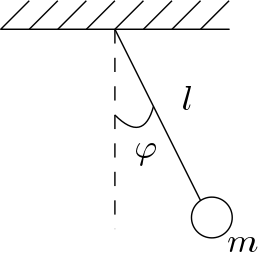
\includegraphics[height=4cm]{matoscill.png}
\qquad \qquad \qquad
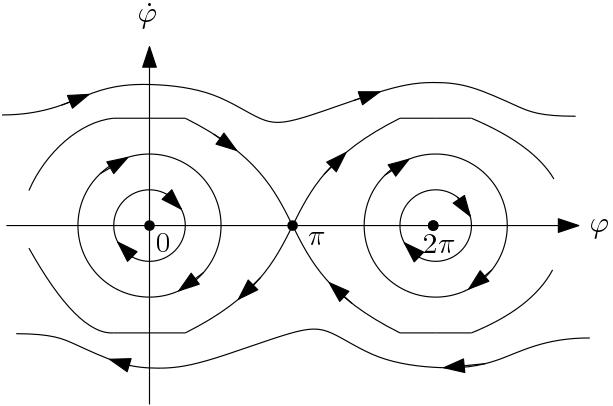
\includegraphics[height=5cm]{phaseportrait.png}
\end{figure}
\begin{flalign*}
& 1) h < - mgl \quad \varnothing &\\
& 2) h = - mgl, \quad \varphi = 0, \;\varphi = 2\pi \text{ --- равновесие} &\\
& 3) -mgl < h < mgl \text{ --- колебания} &\\
& 4) h = mgl \text{ --- либо равновесие $\varphi = \pi$, либо движение к $\varphi = \pi$} &\\
& 5) h > mgl \text{ --- вращение} &\\
\end{flalign*}
\end{xmp}

\begin{xmp}[Маятник во вращающейся плоскости]
\begin{flalign*}
& n = 1, q = \varphi &\\
& T = \frac{m}{2} \v v^2 = \frac{m}{2}\left( r^2\dot \varphi^2 + \omega^2r^2\sin^2 \varphi \right) &\\
& \Pi = - mgr\cos \varphi &\\
& L = T - \Pi, \quad \pd{L}{t} = 0 \Rightarrow T_2 \underbrace{- T_0 + \Pi}_{\Pi^*} = const &\\
& \Pi^* = - mgr\cos \varphi - \frac{m}{2} r^2 \omega^2 \sin^2 \varphi &\\
& \pd{ \Pi^*}{\varphi} = mgr\sin \varphi - \frac{1}{2}mr^2\omega^2 \sin 2\varphi = mr\sin \varphi(g - r\omega^2\sin\varphi) = 0 \Leftrightarrow &\\
& \Leftrightarrow 
\left[
\begin{array}{l}
\varphi = 0 \\
\varphi = \pi \\
\varphi = \pm \arccos \frac{g}{r\omega^2} = \varphi_0, \omega^2 > \frac{g}{2} \\
\end{array}
\right. &\\
& \frac{\partial^2 \Pi^*}{\partial \varphi^2} = mgr\cos\varphi - mr^2\omega^2\cos2\varphi &\\
& \left.\frac{\partial^2 \Pi^*}{\partial \varphi^2}\right|_{\varphi = 0} = mr(g - r\omega^2) \gtrless 0 \quad \omega^2 \lessgtr \frac{g}{r} &\\
& \left.\frac{\partial^2 \Pi^*}{\partial \varphi^2}\right|_{\varphi = \pi} = -mr(g + r\omega^2) < 0, &\\
& \left.\frac{\partial^2 \Pi^*}{\partial \varphi^2}\right|_{\varphi = \varphi_0} = mgr\frac{g}{r \omega^2} - mr^2\omega^2 \left(2 \frac{g^2}{r^2\omega^4} - 1\right) = mr\omega^2\left( r - \frac{g^2}{2\omega^4} \right) < 0&\\
\end{flalign*}
\begin{figure}[H]
\centering
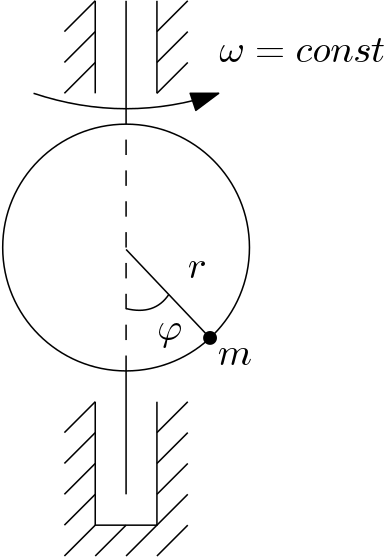
\includegraphics[height=5cm]{rotatingosc.png}
\qquad \qquad \qquad
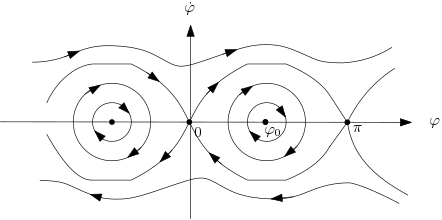
\includegraphics[height=4cm]{otherphaseportrait.png}
\end{figure}
\end{xmp}